\documentclass[border=4pt]{standalone}

\usepackage{amsmath}
\usepackage{tikz}
\usepackage{mathdots}
\usepackage{yhmath}
\usepackage{cancel}
\usepackage{color}
\usepackage{siunitx}
\usepackage{array}
\usepackage{multirow}
\usepackage{amssymb}
\usepackage{gensymb}
\usepackage{tabularx}
\usepackage{booktabs}
\usetikzlibrary{fadings}
\usetikzlibrary{patterns}


\begin{document}



\tikzset{every picture/.style={line width=0.75pt}} %set default line width to 0.75pt        

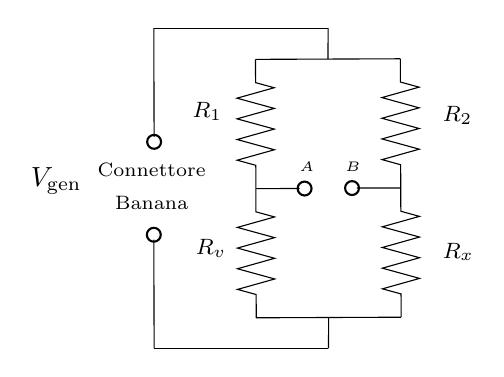
\begin{tikzpicture}[x=0.75pt,y=0.75pt,yscale=-1,xscale=1]
%uncomment if require: \path (0,300); %set diagram left start at 0, and has height of 300

%Shape: Resistor [id:dp7838028787100733] 
\draw   (369.3,75.97) -- (369.33,87.18) -- (378.31,89.64) -- (360.38,94.67) -- (378.34,99.6) -- (360.41,104.63) -- (378.37,109.56) -- (360.43,114.59) -- (378.4,119.52) -- (360.46,124.55) -- (369.44,127.02) -- (369.47,138.22) ;
%Shape: Resistor [id:dp10409637467714616] 
\draw   (369.47,138.22) -- (369.51,149.43) -- (378.49,151.9) -- (360.55,156.93) -- (378.52,161.86) -- (360.58,166.89) -- (378.54,171.82) -- (360.61,176.85) -- (378.57,181.78) -- (360.64,186.81) -- (369.62,189.27) -- (369.65,200.48) ;
%Straight Lines [id:da11373267650453145] 
\draw    (299.5,76.25) -- (369.3,75.97) ;
%Straight Lines [id:da3141812151950649] 
\draw    (299.85,200.76) -- (369.65,200.48) ;
%Shape: Resistor [id:dp6557995768098865] 
\draw   (299.5,76.25) -- (299.53,87.46) -- (308.51,89.92) -- (290.58,94.95) -- (308.54,99.88) -- (290.61,104.91) -- (308.57,109.84) -- (290.63,114.87) -- (308.6,119.8) -- (290.66,124.83) -- (299.64,127.3) -- (299.67,138.51) ;
%Shape: Resistor [id:dp988187811158096] 
\draw   (299.67,138.51) -- (299.71,149.71) -- (308.69,152.18) -- (290.75,157.21) -- (308.71,162.14) -- (290.78,167.17) -- (308.74,172.1) -- (290.81,177.13) -- (308.77,182.06) -- (290.83,187.09) -- (299.82,189.55) -- (299.85,200.76) ;
%Straight Lines [id:da4657385020242546] 
\draw    (348.35,138.25) -- (369.47,138.22) ;
\draw [shift={(346,138.25)}, rotate = 359.94] [color={rgb, 255:red, 0; green, 0; blue, 0 }  ][line width=0.75]      (0, 0) circle [x radius= 3.35, y radius= 3.35]   ;
%Straight Lines [id:da6331364906320349] 
\draw    (299.67,138.51) -- (320.8,138.48) ;
\draw [shift={(323.15,138.48)}, rotate = 359.94] [color={rgb, 255:red, 0; green, 0; blue, 0 }  ][line width=0.75]      (0, 0) circle [x radius= 3.35, y radius= 3.35]   ;
%Straight Lines [id:da5562408882729599] 
\draw    (334.5,61.25) -- (334.4,76.11) ;
%Straight Lines [id:da8704675373012849] 
\draw    (334.75,200.62) -- (334.65,215.48) ;
%Straight Lines [id:da8099858477231627] 
\draw    (250.5,61.25) -- (334.5,61.25) ;
%Straight Lines [id:da728765023988192] 
\draw    (250.65,215.48) -- (334.65,215.48) ;
%Straight Lines [id:da033538017554630706] 
\draw    (250.51,163.1) -- (250.65,215.48) ;
\draw [shift={(250.5,160.75)}, rotate = 89.84] [color={rgb, 255:red, 0; green, 0; blue, 0 }  ][line width=0.75]      (0, 0) circle [x radius= 3.35, y radius= 3.35]   ;
%Straight Lines [id:da5295595601182028] 
\draw    (250.5,61.25) -- (250.64,113.63) ;
\draw [shift={(250.65,115.98)}, rotate = 89.84] [color={rgb, 255:red, 0; green, 0; blue, 0 }  ][line width=0.75]      (0, 0) circle [x radius= 3.35, y radius= 3.35]   ;

% Text Node
\draw (341.5,124.4) node [anchor=north west][inner sep=0.75pt]  [font=\tiny]  {$B$};
% Text Node
\draw (319.5,124.4) node [anchor=north west][inner sep=0.75pt]  [font=\tiny]  {$A$};
% Text Node
\draw (388.5,97.4) node [anchor=north west][inner sep=0.75pt]  [font=\footnotesize]  {$R_{2}$};
% Text Node
\draw (268,95.9) node [anchor=north west][inner sep=0.75pt]  [font=\footnotesize]  {$R_{1}$};
% Text Node
\draw (388.5,163.4) node [anchor=north west][inner sep=0.75pt]  [font=\footnotesize]  {$R_{x}$};
% Text Node
\draw (269.5,161.9) node [anchor=north west][inner sep=0.75pt]  [font=\footnotesize]  {$R_{v}$};
% Text Node
\draw (221.5,125) node [anchor=north west][inner sep=0.75pt]   [align=left] {\begin{minipage}[lt]{40.035000000000004pt}\setlength\topsep{0pt}
\begin{center}
{\scriptsize Connettore }\\{\scriptsize Banana}
\end{center}

\end{minipage}};
% Text Node
\draw (190,127) node [anchor=north west][inner sep=0.75pt]    {$V_{\text{gen}}$};


\end{tikzpicture}


\end{document}
